\begin{frame}
  \frametitle{Motivation}
 \textblockorigin{0.0cm}{2.0cm}
 
 \begin{textblock*}{11cm}(1.0cm,0.8cm)
 \begin{itemize}
     \item Staus quo in nordic countries
     \begin{itemize}
      \item Overcrowding and limited functionality of manual mobile networks
      \item Interruption of calls when entering another cell area
      \item High cross-border traffic but incompatible technologies
     \end{itemize}
    \end{itemize}
 
 \vspace{0.5cm}
 
   \begin{itemize}
     \item Target state
      \begin{itemize}
	\item Same services as landline
        \item Automated handover of calls between cells
        \item National and international roaming
      \end{itemize}
    \end{itemize}
   \end{textblock*}
    
   \begin{textblock*}{11cm}(1.0cm,5.5cm)
   \begin{center}
     $\Rightarrow$ National telephone operators from Denmark, Finnland, Norway\\and Sweden decided to develop a mobile
phone standard collaboratively
    \end{center} 
   \end{textblock*}
   
  \begin{textblock*}{2.2cm}(11cm,2.0cm)
   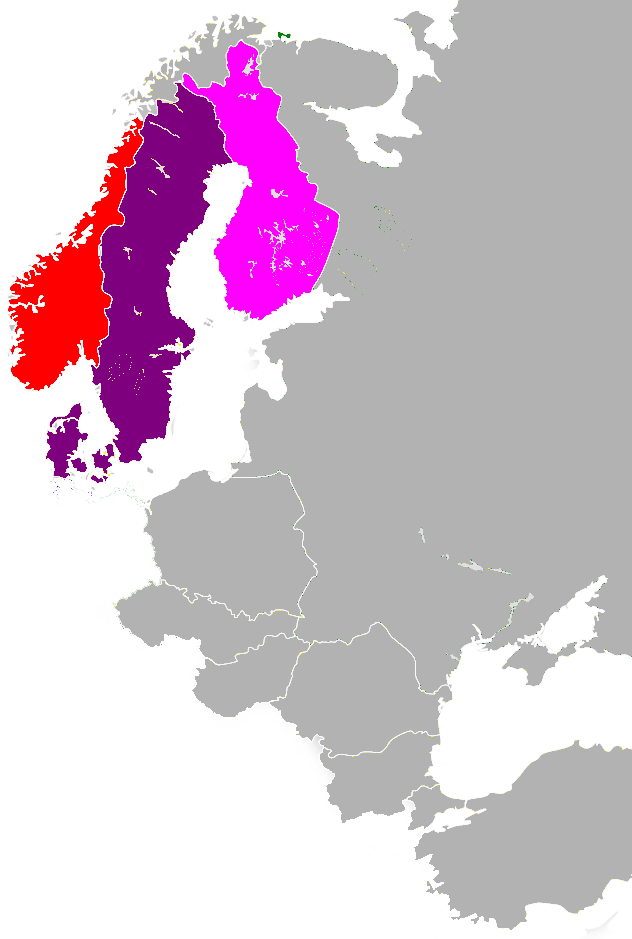
\includegraphics[width=1\columnwidth]{./pictures/0GNordicCountries.png}
  \end{textblock*}
\end{frame}

\begin{frame}
  \frametitle{Negotiation and diffusion}
  \textblockorigin{0.0cm}{2.0cm}
  
  \begin{tikzpicture}
      \node[anchor=south west,inner sep=0] (timeline) at (0,0) {
      \begin{chrono}[10]{1969}{1986}{3ex}{\textwidth}
	\event{1969}{Identification of common standard advantages}
	\event{1970}{First meeting of operator representatives}
	\event{1971}{Fourteen operational requirements}
	\event[1981]{1982}{NMT-450 release (on time)}
	\event{1985}{Largest cellular phone system world-wide}
	\event{1986}{NMT-900 release}
      \end{chrono}
    };
    \only<2>{
      \begin{scope}[x={(timeline.south east)},y={(timeline.north west)}]
          \draw[red,ultra thick,rounded corners, fill=red!60, opacity=.7] (0.00,0.035) rectangle (0.1,0.10);
          \node[anchor=north west,color=red!60,inner sep=0] (timeline) at (0,0) {\small{Pre-standardisation}};
          \draw[blue,ultra thick,rounded corners, fill=blue!60, opacity=.7] (0.51,0.035) rectangle (0.1,0.10);
          \node[anchor=north west,color=blue!60,inner sep=0] (timeline) at (0.25,0) {\small{Standard Production}};
          \draw[green,ultra thick,rounded corners, fill=green!60, opacity=.7] (0.7,0.035) rectangle (0.51,0.10);
          \node[anchor=north west,color=green!60,inner sep=0] (timeline) at (0.52,0) {\small{Standard Diffusion}};
      \end{scope}
    }
  \end{tikzpicture}
  
  \begin{textblock*}{11cm}(1.0cm,5.95cm)
     $\Rightarrow$ Unexpected, international success of NMT standard
  \end{textblock*}
  
  \begin{textblock*}{2.2cm}(11cm,2.0cm)
    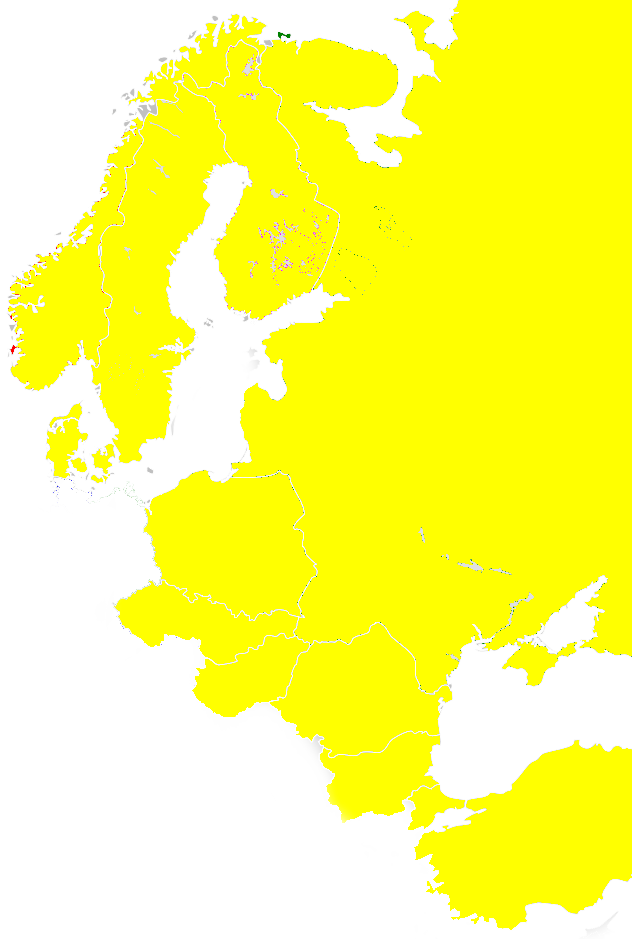
\includegraphics[width=1\columnwidth]{./pictures/1GNordicCountries.png}
  \end{textblock*}
    
\end{frame}

\begin{frame}
  \frametitle{Success factors}
  
  \begin{itemize}
    \item \textbf{Market orientation}
      \begin{itemize}
       \item Market pull
       \item Critical market size
       \item Little involvement of governements/national institutes
      \end{itemize}
  \end{itemize}

  \begin{itemize}
    \item \textbf{Comitee composition}
      \begin{itemize}
	\item Culture of cooperation
	\item Small working groups, members with similar technical background
	\item Intense relationship with manufactorers
      \end{itemize}
  \end{itemize}

  \begin{itemize}
    \item \textbf{Neutral manufactorer treatment}
      \begin{itemize}
       \item Focus on interface specification
       \item Open standard without any license fees
       \item Economics of scale       
      \end{itemize}
  \end{itemize}
\end{frame}
